\documentclass[MasterThesisMain.tex]{subfiles}
\begin{document}
	\chapter{Experimental method}\label{experimentalmethod}
	
In this chapter, a general outline of polymer classification will be outlined with the addition of a description of the polymers used in the solvent vapour annealing experiments. The spectrometer setup will be introduced and the necessary information related to how the spectrometer measures the reflectance of the thin films and the experimental measurement protocol will be outlined. The reflectance data fitting will be explained and the chapter will close with a brief description of the solvent vapour annealing process. 
	
\section{Polymers}
Polymers are long chains of molecular units called monomers, linked together by covalent bonds. Homopolymers are polymers built of one type of monomer repeating, where diblock copolymers are built up of two types of monomers, an A monomer block and B monomer block. 

Polymers can also be expressed by the degree of polymerisation, $N$, which characterises the average number of monomer units in the chain. It is defined as:

\begin{equation}
N = \frac{\bar{M}_n}{\bar{m}},
\end{equation}
where $\bar{M}_n$ is the number average molecular weight and $\bar{m}$ is the monomer molecular weight. The polymerisation of a diblock copolymer is the sum of the individual block polymerisation, $N = N_A + N_B$. The number average molecular weight is defined as:
\begin{equation}
\bar{M}_n = \frac{\sum N_iM_i}{\sum N_i} = \sum x_iM_i,
\end{equation}      
where $x_i = \frac{N_i}{\sum N_i}$ is the fraction of the number of chains with a corresponding size range $i$ and $M_i$ is mean molecular weight in the size range $i$. The weight average molecular weight for a polymer is defined as:
\begin{equation}
\bar{M}_w=\frac{\sum N_iM_i^2}{\sum N_iM_i},
\end{equation}
where $N_i$ is the number of polymers with weight $M_i$. There is a dispersion of different polymer sizes in a solution, this dispersion is called the polydispersion index of the polymer and is expressed as:

\begin{equation}
PDI = \frac{\bar{M}_w}{\bar{M}_n},
\end{equation} 

where $\bar{M}_w$ is the weight average molecular weight and $\bar{M}_n$ is the number average molecular weight \cite{strobl2007physics}.

The diblock copolymers can be further described by the volume fraction $f$ that the different blocks take up and the Flory-Huggins interaction parameter $\chi$ which describes the degree of incompatibility between the two polymers. The volume fraction of A and B blocks are respectively:

\begin{equation}
f_A = \frac{V_A}{V_{total}} \quad f_B=\frac{V_B}{V_{total}}.
\end{equation}

The Flory-Huggins interaction parameter is determined experimentally and expressed as:

\begin{equation}
\chi(T) = \frac{\chi_H}{T} + \chi_S,
\end{equation} 
where $\chi_H$ is due to enthalpy and $\chi_S$ is due to entropy. Chemically dissimilar polymers tend to display a larger $\chi$ value than chemically similar \cite{BCPthermo}\cite{FHpolymer}.

Polymers are found in different physical states, the most common being in a glass or rubber state. A glassy state is described as amorphous since the structure resembles both a liquid and a solid and this state is found below the polymers glass transition temperature $T_g$ of the polymer. A polymer can melt into a viscous state, this state is its rubber state. This state is found above the polymers glass transition temperature \cite{petty2008molecular}. 

Micro-phase segregation of diblock copolymers is understood as a chemical incompatibility between the different blocks in the block copolymer. The Flory-Huggins interaction parameter $\chi_{AB}$ and the fraction composition of the copolymer $f_A$/$f_B$ are used to define the morphology of the diblock copolymer. The Flory-Huggins interaction parameter describes the free-energy cost per monomer of contacts between the A and B monomers. A positive interaction parameter indicates a net repulsion between the A and B monomers, and a negative interaction parameter indicates mixing. The covalent bond plays a role in the morphology because it prevents macro-phase separation between block A and block B of the diblock copolymer \cite{designpolymers}. The theoretical phase diagram of a diblock copolymer is shown to the left in figure \ref{fig:blockfase} and the experimental phase diagram for polystyrene-b-polyisoprene is shown to the right in figure \ref{fig:blockfase}. Diblock copolymers can be found in a variety of complex morphologies as seen in figure \ref{fig:blockfase}. The modelling and fitting of the homopolymers and diblock polymers will assume that the polymers are in a lamellar morphology denoted as L. The self-assembling properties of the diblock copolymers depend on the mobility of the polymer chains before structural reorganisation can proceed. This is normally done by thermal treatments above the glass transition temperature $T_g$ of the polymer, but with high molar mass systems long annealing times are needed \cite{SVABCP}.

\begin{figure}[H]
\centering
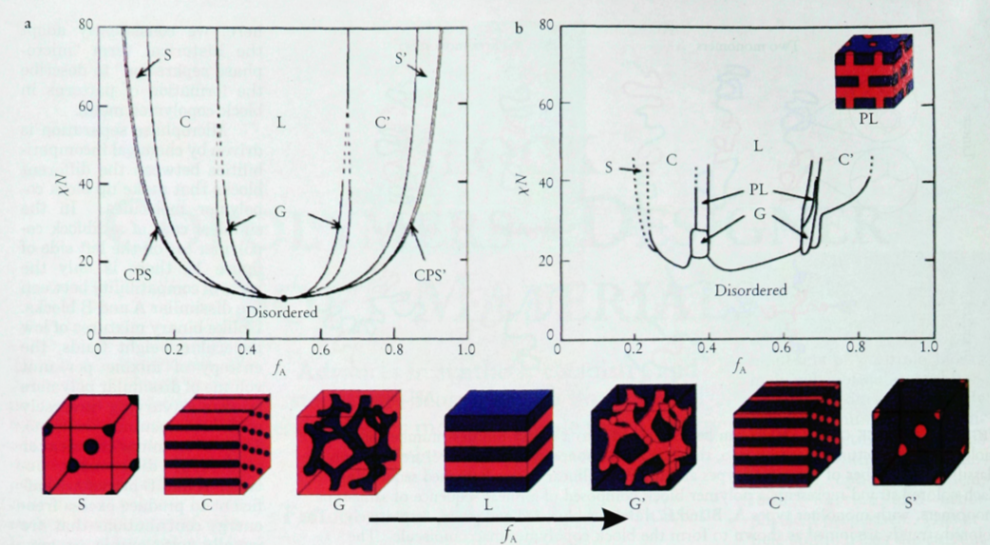
\includegraphics[width = \textwidth]{PSPIphase.png}
\caption{The theoretical phase diagram is shown to the left and the experiment phase diagram for polystyrene-b-polyisoprene is shown to the right. The product of the interaction parameter and the degree of polymerisation as a function of polymer composition of the A block is plotted in both figures. The morphologies the diblock copolymers can be found in are shown below the figures. From left to right the morphologies are spherical, cylindrical, gyroid, and lamellar. The experimental phase diagram for polystyrene-b-polyisoprene resembles the theoretical phase diagram. The experimental phase diagram has one extra morphology denoted as PL \cite{designpolymers}.}
\label{fig:blockfase}
\end{figure}
 

\subsection{Homopolymer Chemistry}
\newcommand\setpolymerdelim[2]{\def\delimleft{#1}\def\delimright{#2}}
\def\makebraces[#1,#2]#3#4#5{%
\edef\delimhalfdim{\the\dimexpr(#1+#2)/2}%
\edef\delimvshift{\the\dimexpr(#1-#2)/2}%
\chemmove{%
\node[at=(#4),yshift=(\delimvshift)]
{$\left\delimleft\vrule height\delimhalfdim depth\delimhalfdim
width0pt\right.$};%
\node[at=(#5),yshift=(\delimvshift)]
{$\left.\vrule height\delimhalfdim depth\delimhalfdim
width0pt\right\delimright_{\rlap{$\scriptstyle#3$}}$};}}


\setpolymerdelim[]
Polystyrene \ce{(C8H8)_N}:
\chemfig{-[@{left,0.3},1.5]C(-[:90]*6(=-=-=-))(-[6]H)-C(-[2]H)(-[6]H)-[@{right,0.8}]}
\makebraces[90pt,30pt]{N}{left}{right}
\bigskip


\setpolymerdelim[]
Polyisoprene \ce{(C5H8)_N}:
\chemfig{-[@{left,0.3},1.5]CH_2-CH=C(-[6]CH_3)-CH_2-[@{right,0.8}]}
\makebraces[10pt,15pt]{N}{left}{right}


\section{Polymer Considerations}
Before commencing solvent vapour annealing some consideration is needed to determine which polymers, which solvent and which substrate should be used. Polystyrene has been chosen as block A of the block copolymer and Polyisoprene has been chosen as block B. Polystyrene is in the glassy phase at room temperature, where polyisoprene is in a rubbery phase at room temperature. The morphology of the block sheds light on how the vapour interacts with the blocks during solvent vapour annealing. The molar mass, polymerisation of both block, polydispersion index, and the interaction parameter between the two blocks is helpful in order to understand what might happen during the solvent vapour annealing process. High molar mass systems are strongly segregated and take longer to come into equilibrium than a lower molar mass system. Interaction between the solvent and the polymers will also give insight into how the morphology could evolve during the solvent vapour annealing.

\begin{table}
	\caption{Relevant values}
\begin{tabular}{ |p{3cm}||p{3cm}|p{3cm}|p{3cm}|  }
 \hline
 \multicolumn{4}{|c|}{Polymer Values} \\
 \hline
    & Polystyrene & Polyisoprene & PS-b-PI\\
 \hline
 $T_g$& $\SI{379}{\kelvin}$   & $\SI{204}{\kelvin}$  &   \\
 $N$&  &  &  \\
 $N_A$&  &  &  \\
 $N_B$&  &  &  \\
 $f_A$ nominal&  &  & $0.5$  \\
 $f_B$ nominal&  &  & $0.5$  \\
 $\bar{M}_n$&  &  &  \\
 $\bar{M}_w$&  &  &  \\
 $PDI$&  &  &  \\
 $\chi$&  &  &  \\
 $n$& $1.60$ & $1.51$ & Unknown\\
 \hline
\end{tabular}
\end{table}


\begin{table}
	\caption{List of polymers used in experiments}
\begin{tabular}{ |p{3cm}||p{2cm}|p{2cm}|p{2cm}|p{2cm}|p{2cm}|  }
 \hline
 \multicolumn{6}{|c|}{Polymer used in experiments} \\
 \hline
 Experiment & Polymer & ID & Spincoat Thickness eq.\ref{eq:spin} & Single point stage static thickness measurement & Single point stage static refractive index\\
 \hline
 Light Source Fluctuation & Polystyrene & 349 & $\approx\SI{200}{\nano\meter}$ & $\SI{280}{\nano\meter}$ & $1.5944$  \\
 SVA Ambient Study & Topsil Blank & N/A & N/A & N/A & N/A  \\
 Polystyrene Swelling & PS  & 348  & $\approx\SI{200}{\nano\meter}$ & $\SI{275}{\nano\meter}$ & $1.5975$  \\
 Polyisoprene Swelling & PI  & 353 & $\approx\SI{200}{\nano\meter}$ & $\SI{301}{\nano\meter}$ & $1.4594$  \\
 Polystyrene-b-Polyiosprene & PS-b-PI & 370 & $\approx\SI{100}{\nano\meter}$ & $\SI{97}{\nano\meter}$ & $1.5659$ \\  
\hline
\end{tabular}
\label{tab:polymers}
\end{table}

\section{Spin Coating thin films}
Spin coating is the deposition method used to fabricate the thin films used in this thesis. This is a wet method where a polymer is dissolved in a solution, then deposited onto the semiconductor wafer, silicon wafer. The silicon wafer is rotated at a fixed low rpm to spread the polymer solution across the wafer. The rpm is increased, spinning off the excess solution and evaporation will leave a thin film with uniform thickness. This method is predicted by the following expression:

\begin{equation}\label{eq:spin}
d = \left(\frac{\eta}{4\pi\rho\omega^2}\right)^{\frac{1}{2}} t^{-\frac{1}{2}},
\end{equation}  
where d is the predicted thickness, $\eta$ the viscosity coefficient of the polymer solution, $\rho$ solution density, $\omega$ angular velocity of the spinning and $t$ is the spinning time \cite{petty2008molecular}. The spin coated block copolymers show defect-rich morphologies due to fast evaporation of the solvent and the polymers being in a thermal non-equilibrium \cite{PosseltBCP}.

\section{Spectrometer Setup}
The experimental setup is comprised of a NanoCalc XR and a Halogen light source(HL-2000-FHSA) seen in figure \ref{fig:speclight}, which can produce wavelengths of \SI{360}{\nano\meter} to \SI{2400}{\nano\meter}. When the samples are being measured they are either placed on the ocean optics single point stage seen in figure \ref{fig:Singlestage} or in the solvent vapour annealing (SVA) experimental chamber seen in figure \ref{fig:SVAchamber} made by the IMFUFA(Indsatsområdet for Studiet af Matematik og Fysik samt deres Funktioner i Undervisning, Forskning og Anvendelser) workshop for small angle x-ray scattering (SAXS) and and grazing incidence small angle x-ray scattering(GISAXS) experiments. The NanoCalc is comprised of a spectrometer and an internal light source as seen in figure \ref{fig:nanocalcsetup}, which can produce wavelengths of \SI{250}{\nano\meter} to \SI{1050}{\nano\meter} and measure thicknesses of \SI{10}{\nano\meter} to \SI{100}{\micro\meter}. The NanoCalc XR is connected to a computer where the NanoCalc software is installed and operated. For the experiments, the halogen light source is used since it has a larger output power than the internal light source of the NanoCalc XR. The larger intensity output is needed when performing experiments in the SVA experimental chamber. The lid of the SVA experimental chamber holds the optical fiber and light passes through a sapphire lens before entering the chamber and illuminates the thin film. The sapphire lens is needed to focus the light upon the thin film due to the distance from the optical fiber to the sample is much greater than the optimal distance of $\SI{4}{\milli\meter}$. Throughout this thesis "with optics" will be used when referring to measurements taken using the SVA experimental chamber, since the light passes through the sapphire lens. "Without optics" refers to taking measurements using the single point stage.  

For experiments done in this thesis, white light is produced by the light source(HL-2000-FHSA), which travels through optical fiber and strikes the sample. The reflected light travels back through the optical fiber and the intensity across wavelengths $\SI{400}{\nano\meter}$-$\SI{1041}{\nano\meter}$ is collected by the spectrometer and is sent to software created in-house and saved to a file and analysed in MATLAB\textsuperscript{\textregistered}. Normally the data collected by the spectrometer is analysed in the NanoCalc software but for this thesis I would like control of how the data is analysed.  
	
	\begin{figure}[ht] 
	  \begin{minipage}[b]{0.5\linewidth}
	    \centering
	    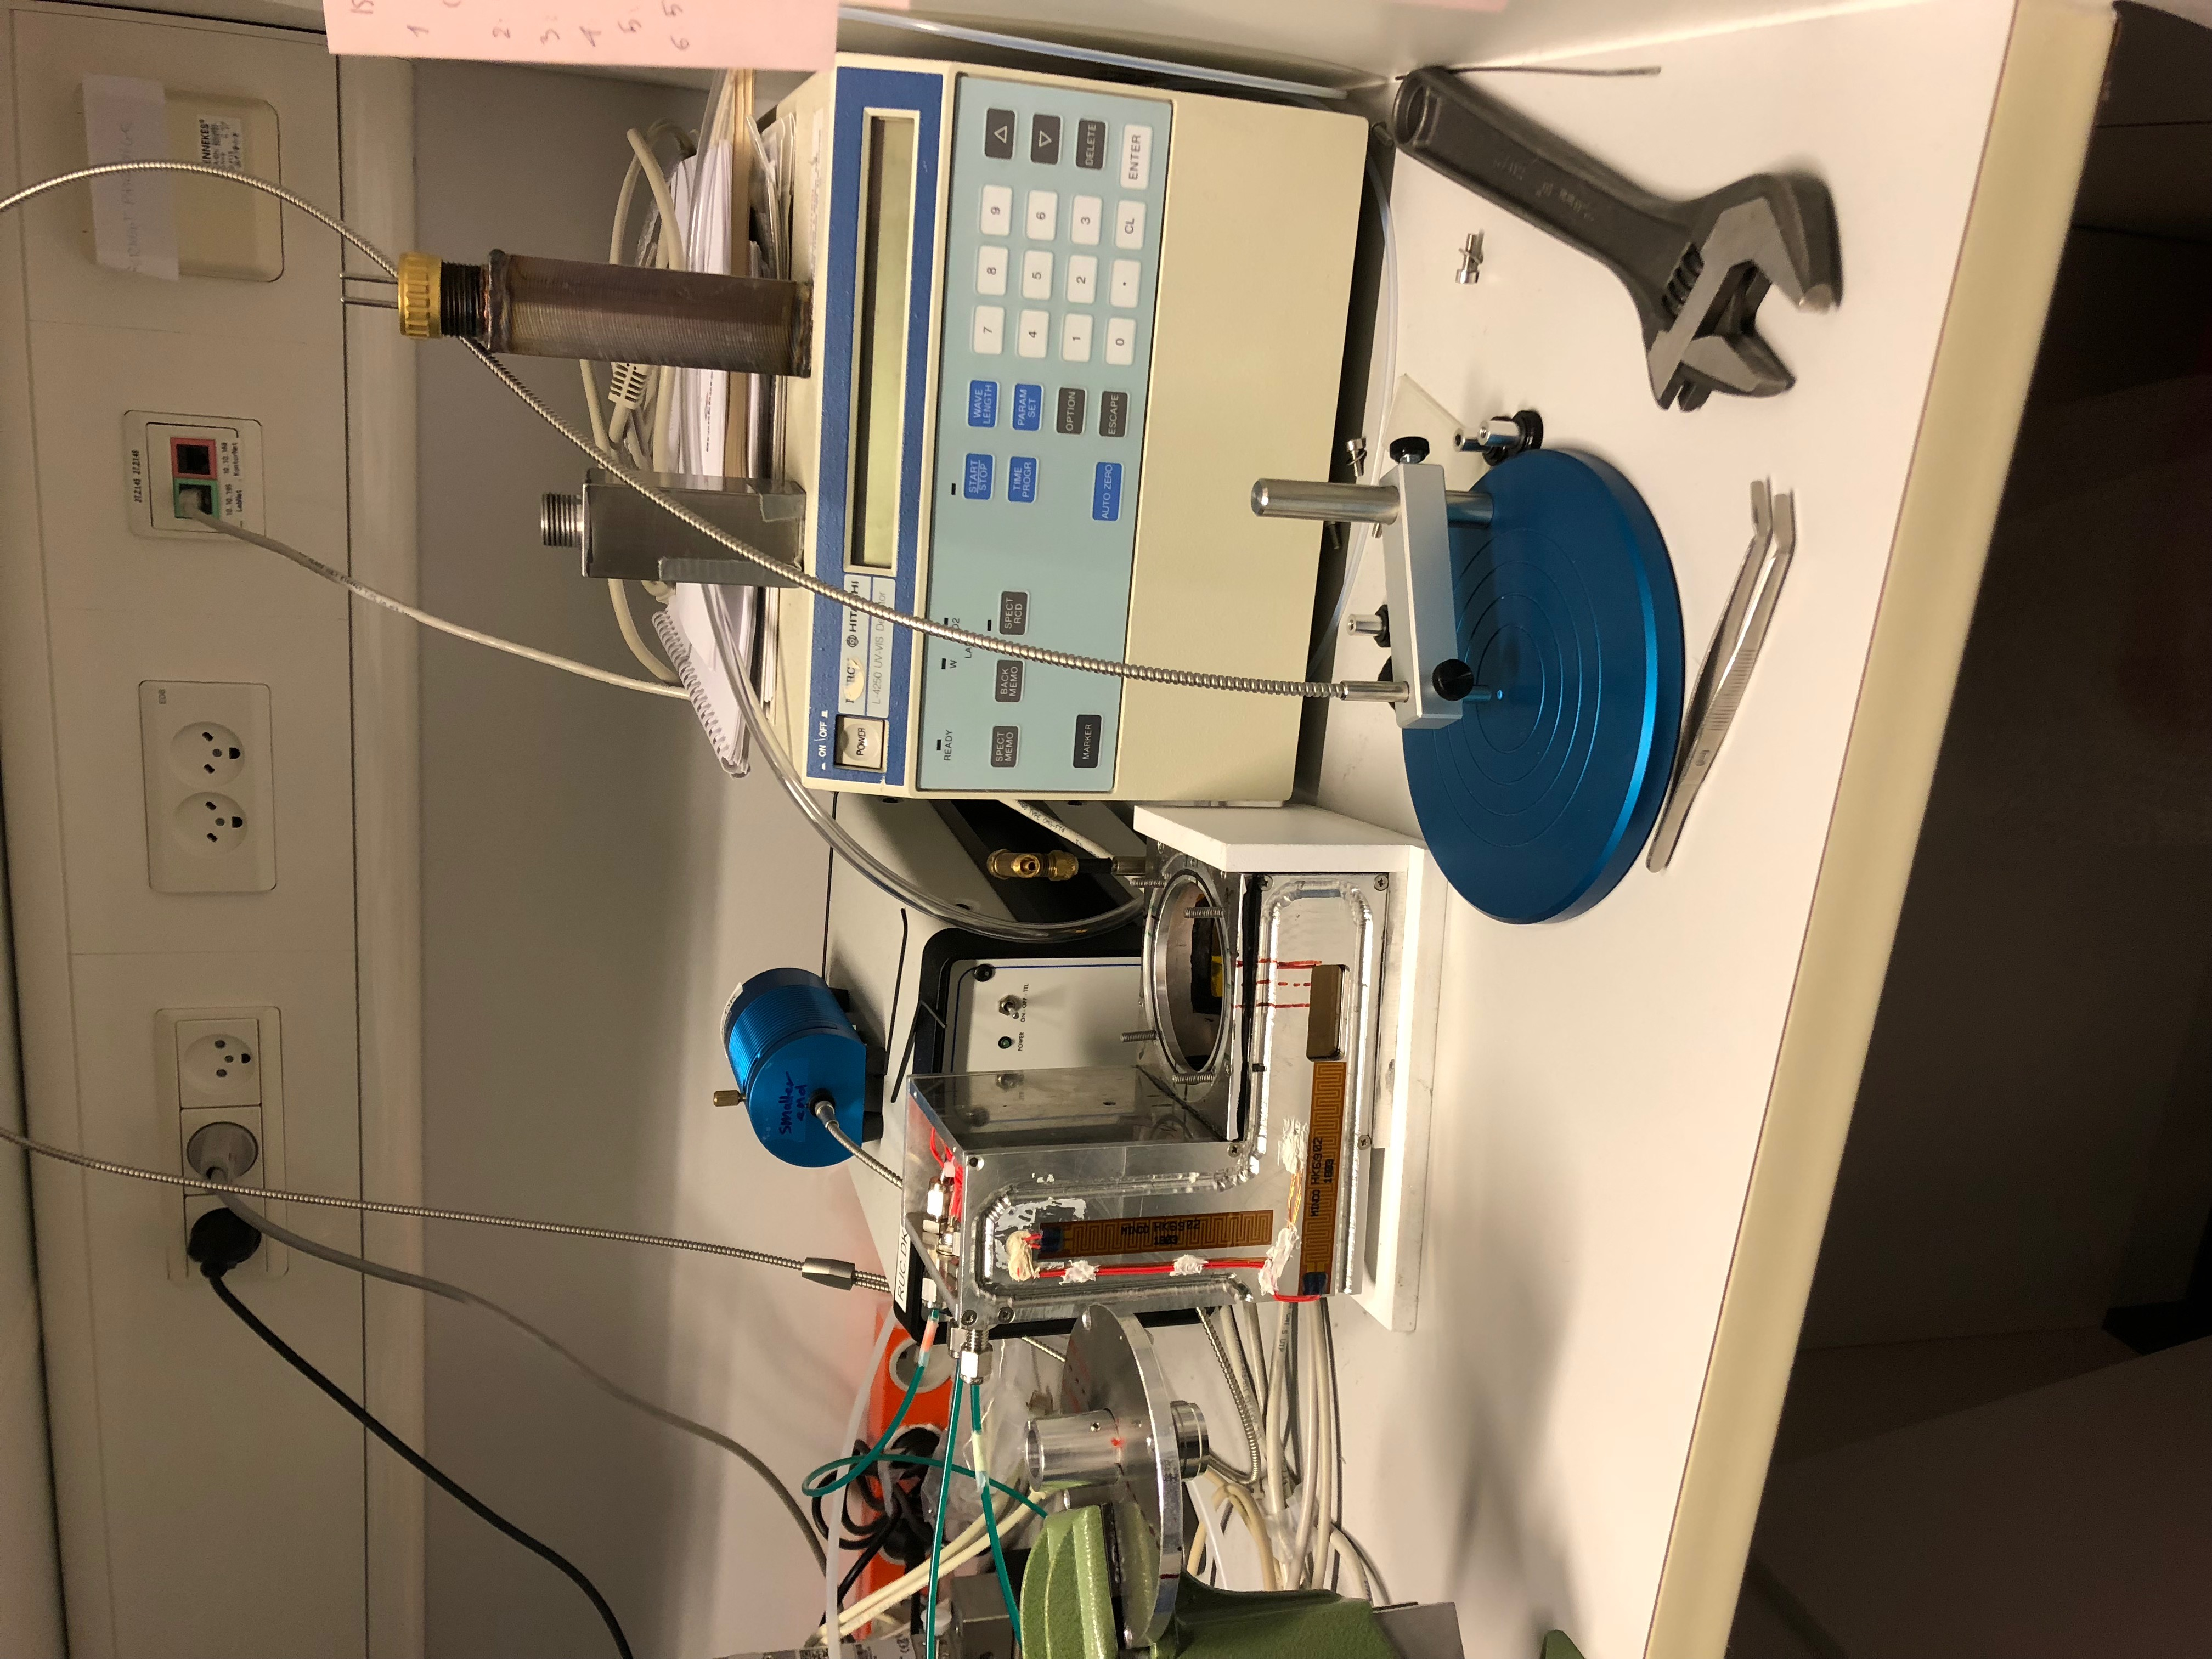
\includegraphics[width=.9\linewidth,angle=-90]{setup1.JPG} 
	    \caption{SVA experiment area}
	    \label{fig:exparea}  
	    \vspace{4ex}
	  \end{minipage}%%
	  \begin{minipage}[b]{0.5\linewidth}
	    \centering
	    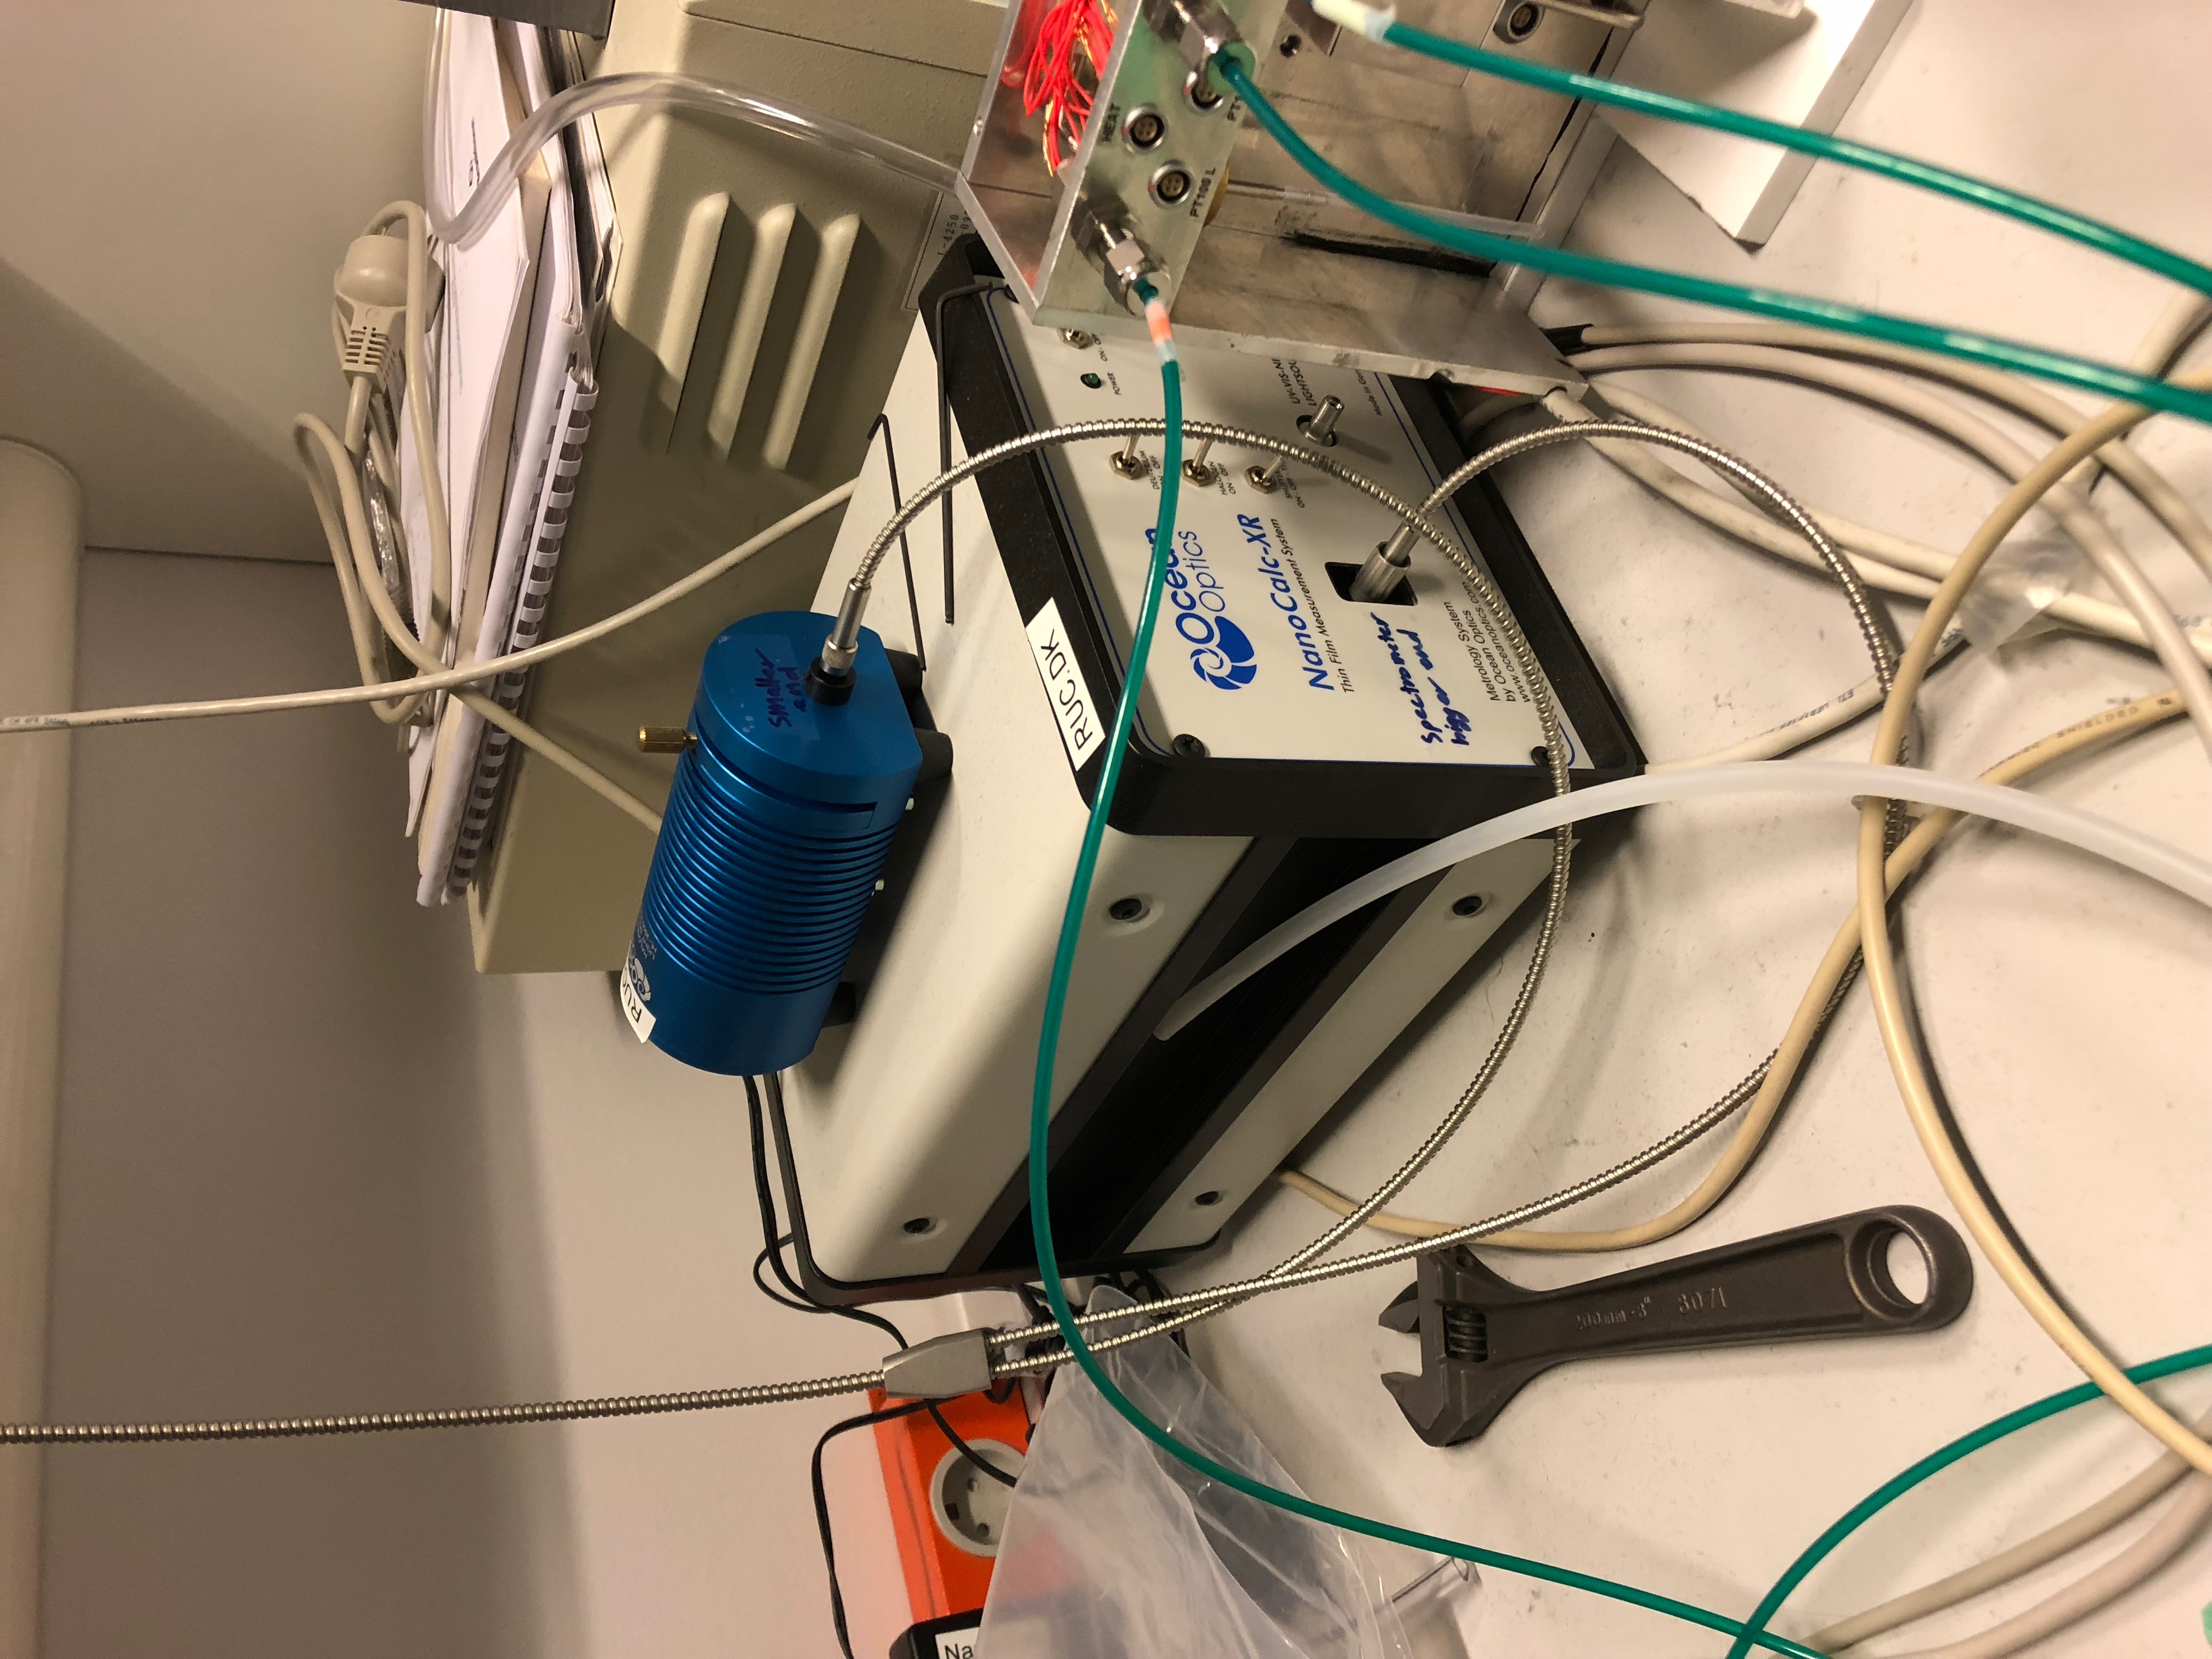
\includegraphics[width=.9\linewidth,angle=-90]{setup2.JPG} 
	    \caption{NanoCalc XR and a Halogen light source(HL-2000-FHSA)}
	    \label{fig:speclight} 
	    \vspace{4ex}
	  \end{minipage} 
	  \begin{minipage}[b]{0.5\linewidth}
	    \centering
	    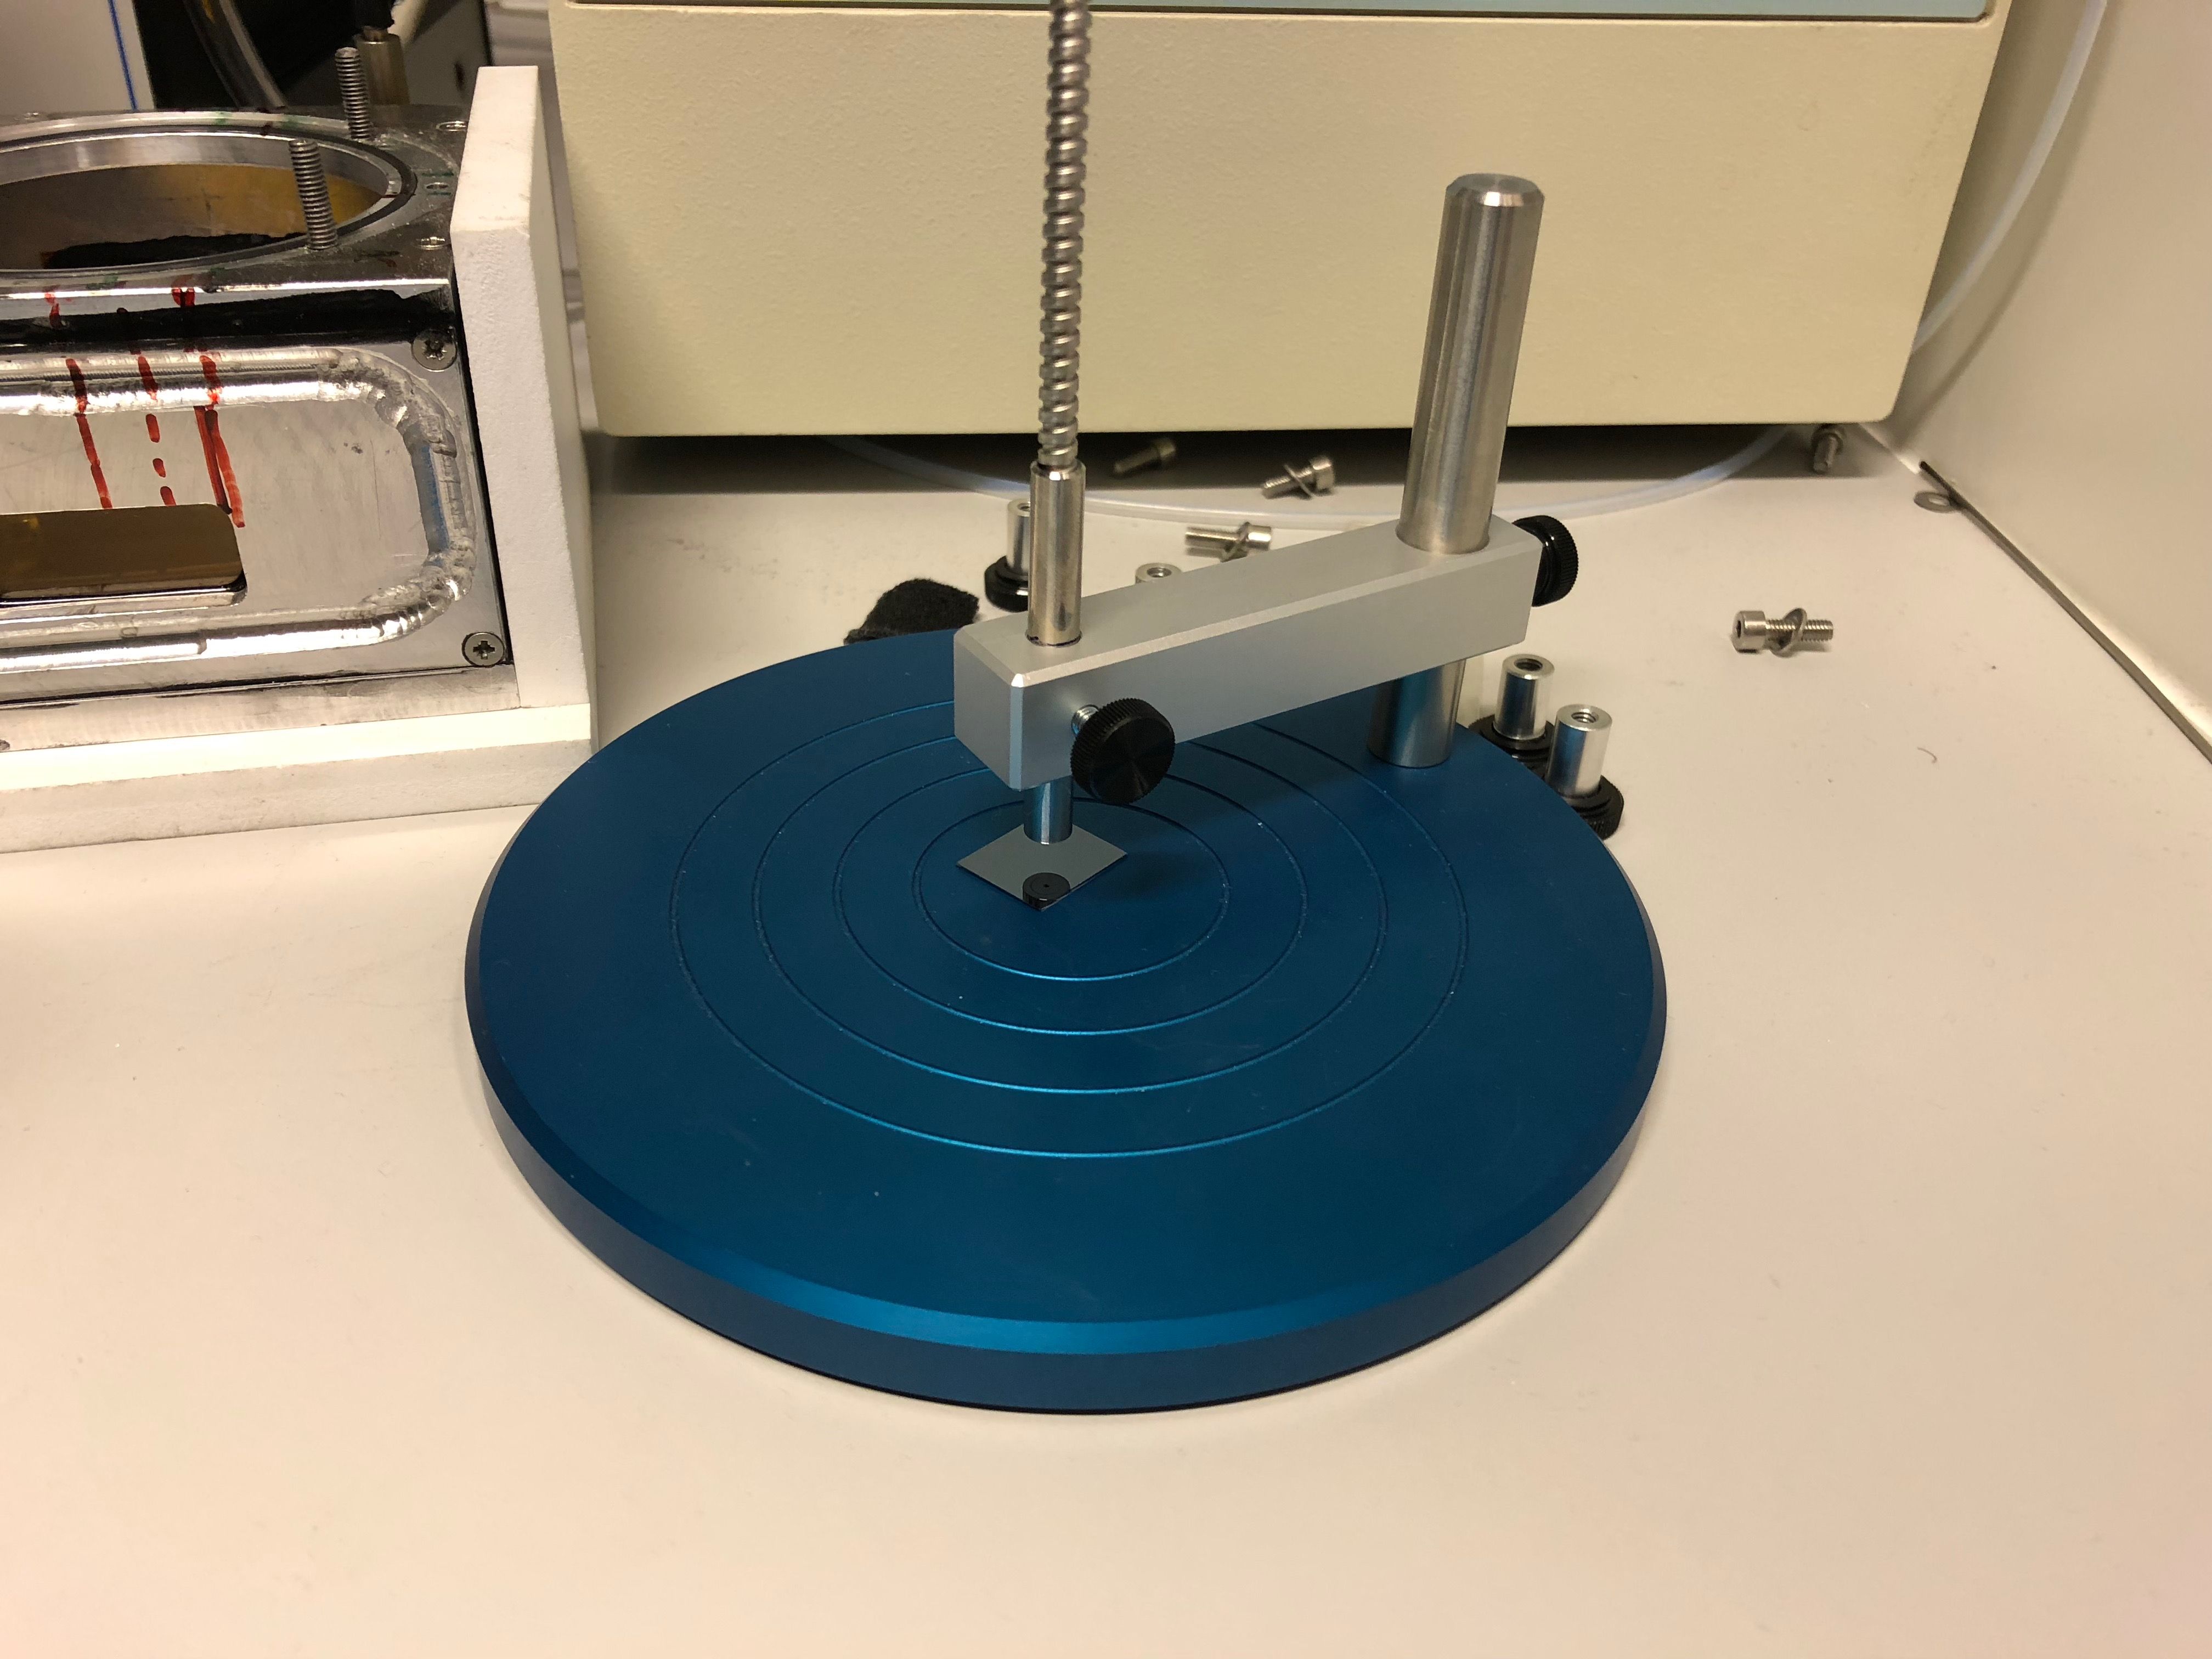
\includegraphics[width=.9\linewidth]{setup3.JPG} 
	    \caption{Single point stage} 
	    \label{fig:Singlestage}
	    \vspace{4ex}
	  \end{minipage}%% 
	  \begin{minipage}[b]{0.5\linewidth}
	    \centering
	    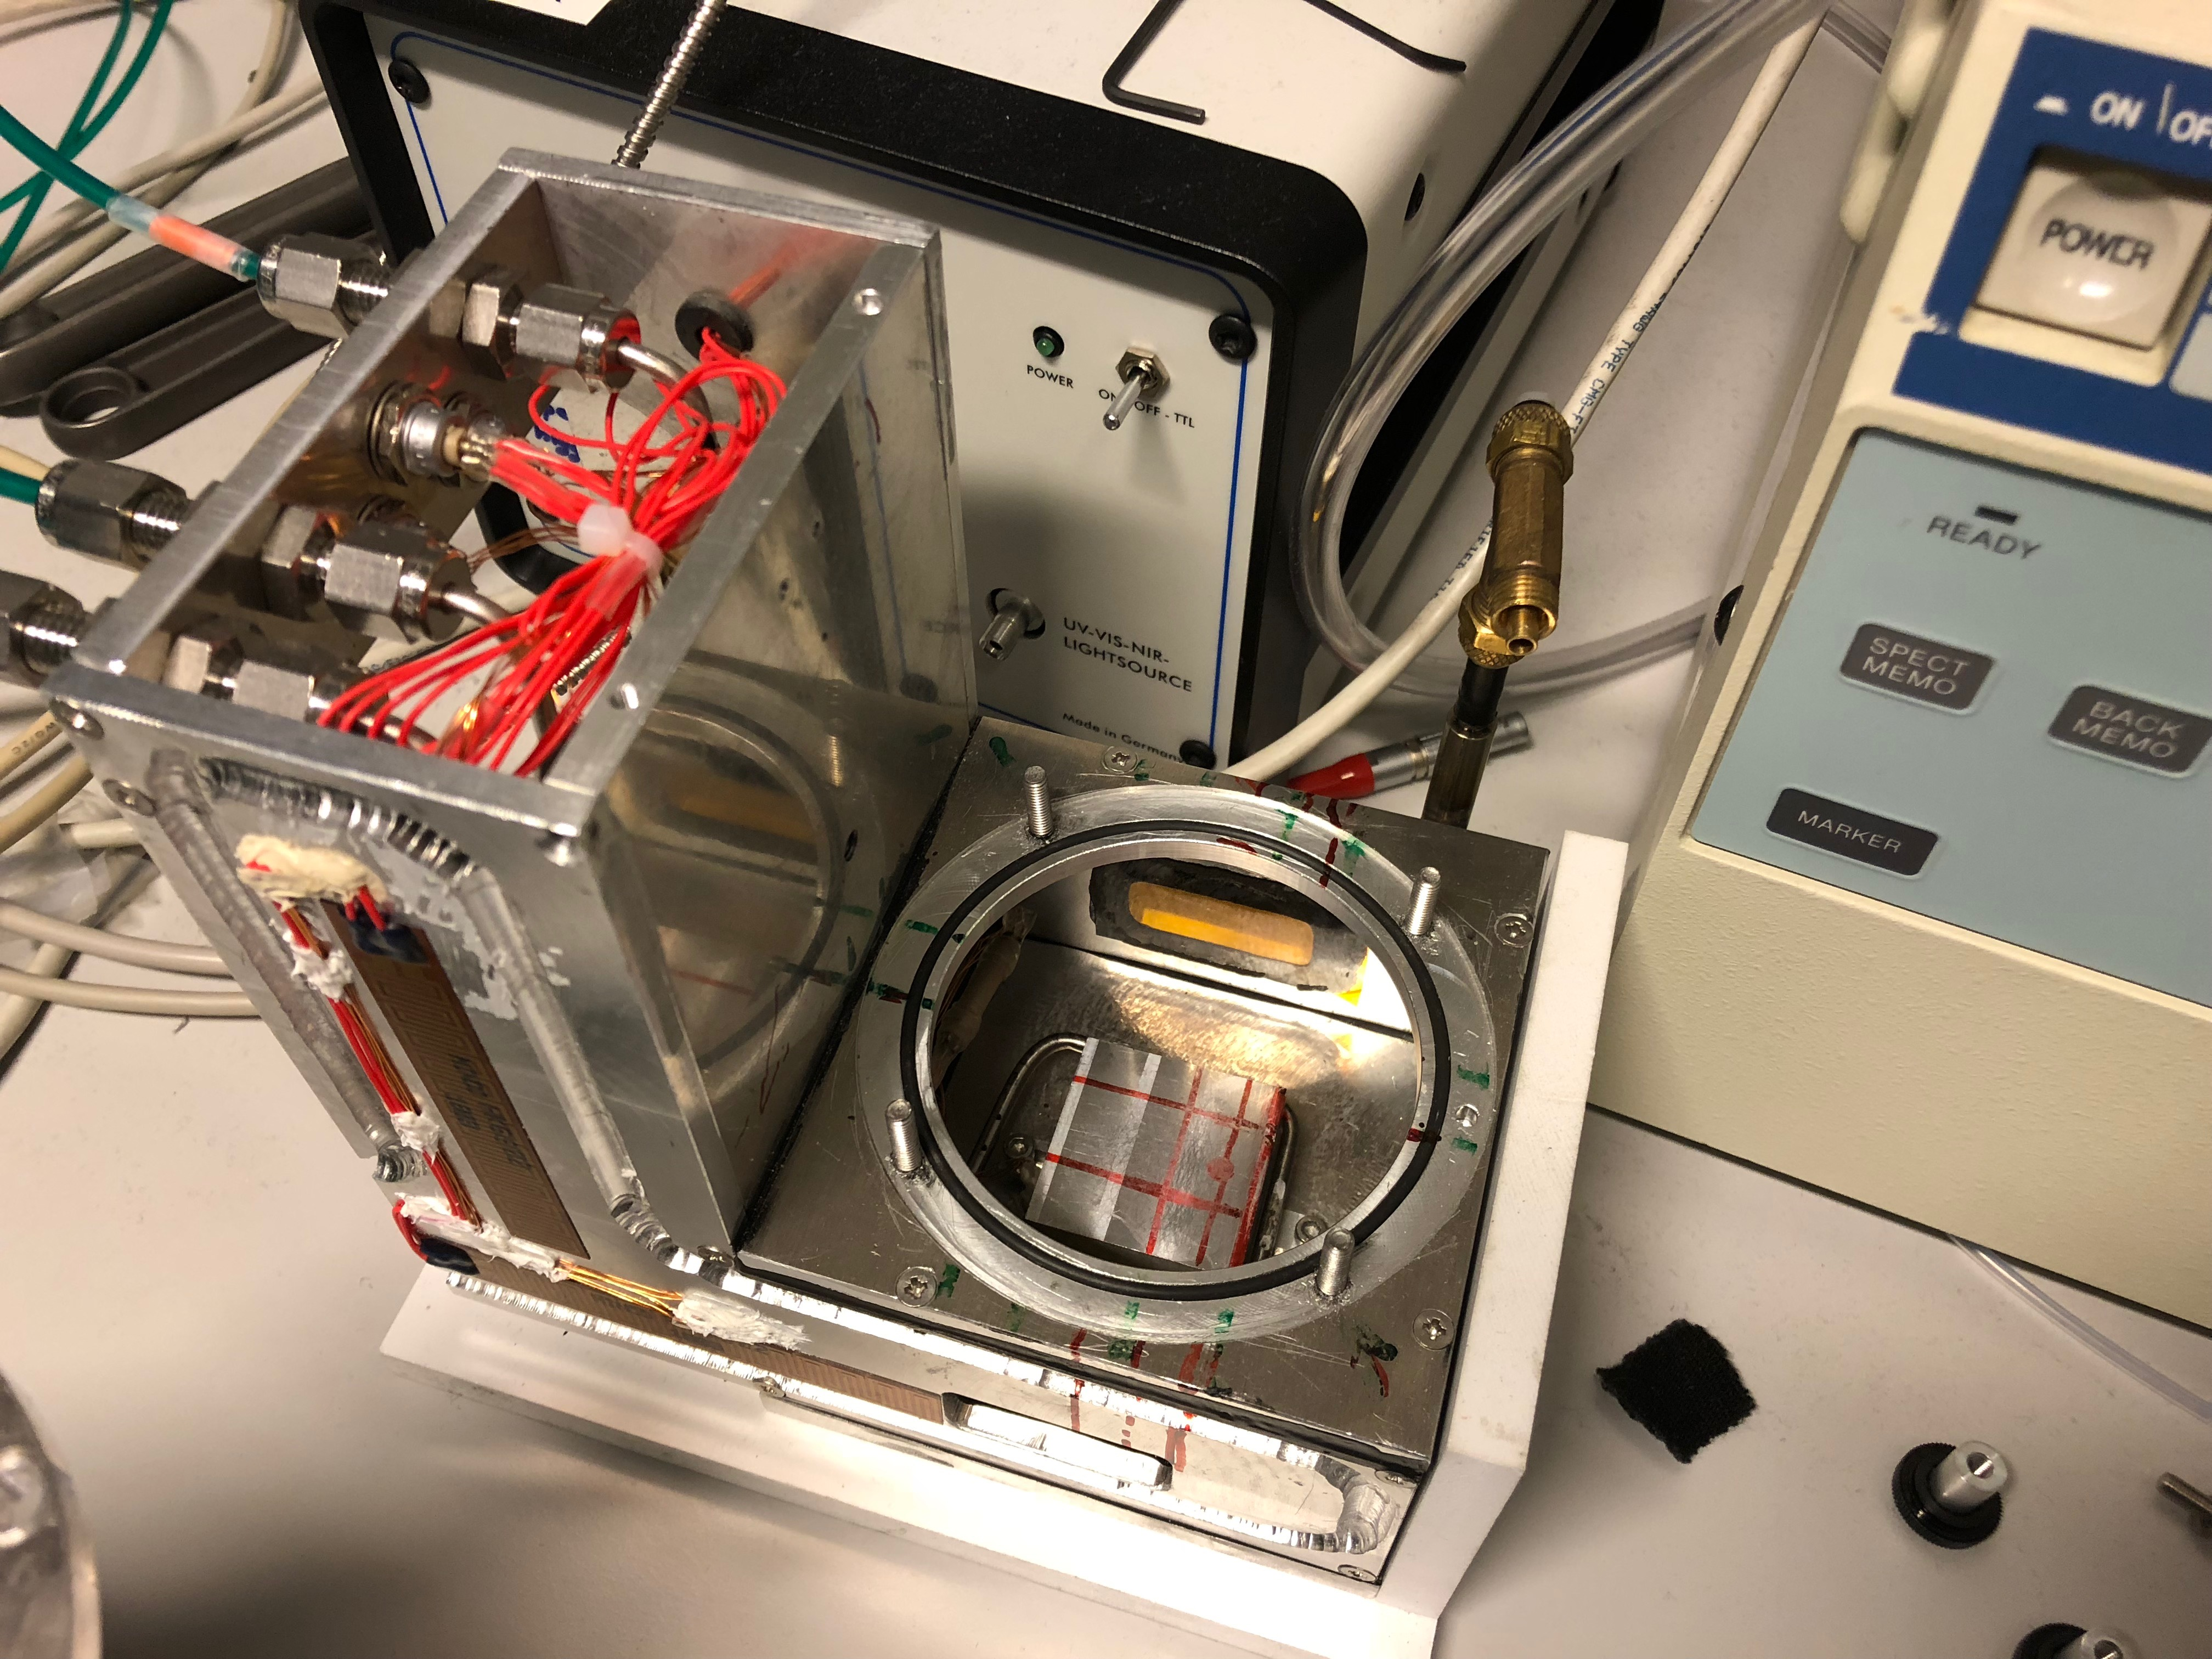
\includegraphics[width=.9\linewidth]{setup4.JPG} 
	    \caption{SVA experimental chamber \break minus lid}
	    \label{fig:SVAchamber} 
	    \vspace{4ex}
	  \end{minipage} 
	\end{figure}
	
	\begin{figure}
	\centering
		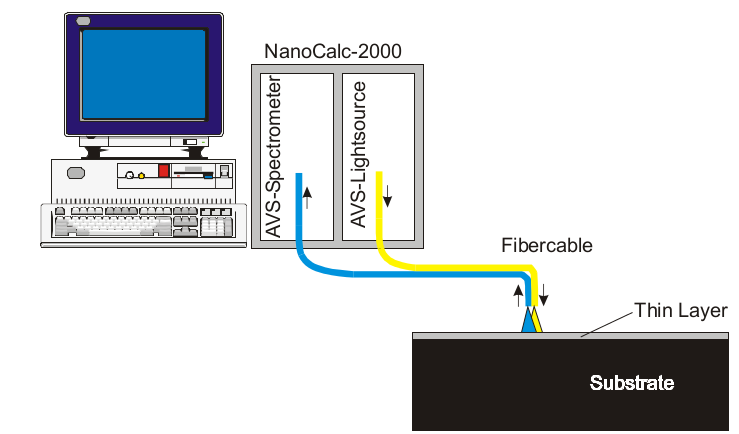
\includegraphics[width=\textwidth]{nanocalcsetup.png}
		\caption{This figure describes the NanoCalc set-up and has been taken from \cite{nanocalcmanual}. Light from a light source travels down the optical fiber illuminating the sample. The reflected light is collected by the optical fiber and analysed in the spectrometer. The spectrometer is connected to the computer by USB and the data is sent to software created in-house and saved to a file and analysed by myself using the Fresnel equations and a fitting protocol.}
		\label{fig:nanocalcsetup}
	\end{figure}
	
\section{Reflectance measurements in the NanoCalc spectrometer}
The NanoCalc spectrometer measures three light intensities which will be called a measurement onwards. The three measurements are the dark measurement (dark), the reference measurement (ref) and the thin-film measurement (meas). The dark measurement is the amount of stray light received by the optical fiber. The reference measurement is the amount of light reflected from a blank silicon wafer and the thin film measurement is the amount of light reflected from the sample $I_{sample}$. From chapter \ref{ch:reflect/trans}, the reflectance of a sample can be expressed as :

\begin{equation}\label{eq:nanocalcrefl}
R_{sample} = \frac{I_{sample}}{I_{incident}}.
\end{equation}

The spectrometer does not measure the intensity of the incident light $I_{incident}$, therefore the reflectance of the substrate $R_{sub}$ is used to isolate the incident light intensity and inserted into equation \ref{eq:nanocalcrefl}. The reflectance of the substrate $R_{sub}$ is used because it can be calculated using the Fresnel equations as described in chapter \ref{ch:fresnelref}.

\begin{align}
R_{sub} = \frac{I_{ref}}{I_{incident}}\\
\implies  I_{incident} = \frac{I_{ref}}{R_{sub}} \label{eq:nanocalcrefl2}.
\end{align}

Inserting equation \ref{eq:nanocalcrefl2} in equation \ref{eq:nanocalcrefl}, the reflectance for the sample is expressed without the incident light intensity as:

\begin{equation}
R_{sample} = \frac{I_{sample}}{I_{ref}} \cdot R_{sub}.
\end{equation}

The intensities $I_{sample}$ and $I_{ref}$ are calculated from the meas, ref and dark. The sample intensity $I_{sample}$ is calculated by the difference of the meas and dark, $I_{sample}=Meas-Dark$ and the intensity $I_{ref}$ is calculated by the difference of the ref and dark, $I_{ref}=Ref-Dark$. The reflectance of the sample is given as:

\begin{equation}
Reflectance = \frac{Meas-Dark}{Ref-Dark} \cdot R_{sub}.
\end{equation}

This is the same expression given in the NanoCalc spectrometer manual \cite{nanocalcmanual}. Through reproduction of the data and curves given by the NanoCalc spectrometer, I can deduce that the reference measurement has already had the dark measurement subtracted, giving the following reflectance expression:

\begin{equation}\label{eq:nanocalcreflect}
Reflectance = \frac{Meas-Dark}{Ref} \cdot R_{sub}.
\end{equation}

Placing equation \ref{eq:nanocalcreflect} equal to the reflectance equations using the Fresnel equations from chapters  \ref{ch:fresnelref}, \ref{ch:fresnel2lay} and \ref{ch:fresnelmulti}, the NanoCalc spectrometer software can fit a thickness of the sample.


\section{Reflectance measurement protocol}
In this section, the experimental protocol for both taking measurements without the optics and with the optics are given. The halogen light source has been turned on 30 minutes prior to taking the measurements and the thin films have had 30 minutes to climatise to room temperature. The single point stage is set up and tested using a reference step wafer of known thickness. The measurement of the dark is different when using the single point stage (Without Optics) and using the solvent vapour annealing chamber (With Optics). Taking a dark measurement, without optics, is done by pointing the optical fiber away from anything that reflects. Taking a dark measurement, with optics, is done by placing a piece of dark cloth into the test chamber and taking a dark measurement with the optical fiber placed into the lid of the chamber. The protocol will be formulated in steps.

\subsection{Without Optics}
\begin{enumerate}
\item Take a continuous reference measurement and adjust the light intensity, such that the reference measurements maximum is $50\%$ of the y-axis.
\item Clear the reference measurement.
\item Take the optic fiber and point it away from anything that can reflect light. Take a dark measurement.
\item Place the optic fiber into ocean optics single point stage. The optic fiber is positioned $4$mm above the single point stage.
\item Place a blank silicon wafer under the optic fiber and take a reference measurement.
\item Save the dark and reference measurement.
\item Place a thin film on a substrate under the optical fiber and take a measurement.  
\end{enumerate}

\subsection{With Optics}
\begin{enumerate}
\item Take a continuous dark measurement with the optic fiber with a dark cloth in the optics where the thin film would lie, and adjust the light intensity, such that the measurement of the dark is at a maximum (100$\%$) of the y-axis.
\item Clear the dark measurement.
\item Place a piece of dark cloth into the test chamber and place the optics into the test chamber. Take a dark measurement.
\item Remove the dark cloth and place a blank silicon wafer into the test chamber and place the optics into the test chamber. Take a reference measurement.
\item Save the dark and reference measurement.
\item Take the optics off the test chamber, remove the blank silicon wafer and place in a thin film sample. Place the optics onto the test chamber. Take a measurement.
\end{enumerate}

\section{Fitting of the reflectance data} \label{sec:fitting}
The mean square error is used when fitting the Fresnel equations to the reflectance measurements. The mean square error is given by:

\begin{equation}
MSE = \frac{1}{n}\sum_{i=1}^{n}\left( Y_i - \hat{Y}_i \right)^2,
\end{equation} 
where $n$ is equal to the amount of data points used, $Y_i$ is the measured value and $\hat{Y}_i$ is the estimated value. The fitting range is from $\SI{450}{\nano\meter}$ to $\SI{900}{\nano\meter}$. The parameters used in the fitting of Fresnel equations are the ambient refractive index $n_0$, the thin film refractive index $n_1$ and the thin film thickness $d_1$. The thickness for the silicon oxide layer is fixed at $\SI{2}{\nano\meter}$ and the complex refractive index values at each wavelength has been taken from Ocean Optics software. Ellipsometry measurements of the blank wafers used has fitted the silicon oxide layer to $\SI{1.7}{\nano\meter}$. I have rounded up to $\SI{2}{\nano\meter}$ for fitting the reflectance measurements. The complex refractive index for the silicon substrate has also been taken from the Ocean Optics software. The complex refractive indices can be found in the appendix \ref{app:dispersion}. During the fitting of the results, real numbers have been used for the refractive indices for the ambient and the thin film. The fitting scripts loop through the three parameter arrays, calculating the mean square error for the measured reflectance data. The scripts find the smallest mean square error value and saves the three parameters associated to the smallest mean square error into an array. The next reflectance measurement is loaded in and the process begins again. The array is then saved into a mat file, which is read when plotting the reflectance data and fitted reflectance curves. These MSE fitting scripts can be seen in the appendix under each of the result sections.

\section{Bronkhorst mass flow meters}
To regulate the solvent vapour annealing process, the experimental setup includes three Bronkhorst mass flow meters. Controlling the vapour flow in different ways is important because this can have an impact in the structuring of the polymers when swelling \cite{SVABCP}. The EL-Flow select(model name:F-201CV-500) has a flow capability for $N_2$ of $\SI{4}{\milli\litre\per\minute}$ to $\SI{750}{\milli\litre\per\minute}$, or $400$ SCCM (Standard centimetre cubed per minute at $\SI{1}{\atmos}$ and $\SI{273}{\kelvin}$). The EL-Flow select(model name:F-201CV-200) has a flow capability for $N_2$ of $\SI{1.6}{\milli\litre\per\minute}$ to $\SI{300}{\milli\litre\per\minute}$, or $200$ SCCM (Standard centimetre cubed per minute at $\SI{1}{\atmos}$ and $\SI{273}{\kelvin}$) \cite{elflow}.

During both swelling processes, the SCCM will be kept constant to $200$ SCCM, meaning that when the nitrogen through the chamber decreases, the nitrogen through the bubbler will increase and the total flow through the mass flow meters will add up to $200$ SCCM.


\section{Solvent Vapour Annealing Process}
The solvent vapour annealing process is divided into two processes, a swelling and a drying process. In the swelling process a dry polymer upon a wafer is placed into the annealing chamber and is subjected to nitrogen gas. Slowly nitrogen gas is decreased and nitrogen gas through a bubbler filled with a solvent, in this thesis toluene, is increased creating vapour in the annealing chamber. When performing SVA, a solvent is chosen that is either neutral or slightly selective towards one of the polymers in the block copolymer. Solvent uptake is also dependent on the physical state of the block copolymer and the block fraction volume. The thin film will swell due to thermodynamic driving forces associated with the entropy of mixing of vapour and polymer blocks. The swelling will continue until the chemical potential of the vapour and the solvent in the thin film is in equilibrium. A diffusion front will arise continuing through the thin film from the vapour interface through to the substrate \cite{SVABCP}. It is published that the vapour pressure is important for the thin film thickness parameter and should be controlled throughout the annealing. The vapour pressure is dependent on the temperature of the solvent and the annealing chamber. The time taken to fully swell is also dependent on how organised the dry thin film is before swelling, which leads to varying swelling time. In a solvent swollen state the mobility of the polymer chains increase and the polymer can move in the volume of the thin film. The molar mass of the polymer plays a role in how fast the polymer self-assembles and an equilibrium state may not be achieved during the swelling. In the drying step, the nitrogen gas flow through the bubbler is decreased, and the direct nitrogen gas flow is increased. The solvent in the thin film is evaporated and the rate in which the solvent evaporates has been seen to have an impact of the nanoscale structure, in the effect of quenching an organised structure. It is documented that both fast and slow evaporation leads to organised structure in block copolymers \cite{SVABCP}. An ordering front forms in the thin film during the evaporation where the thin films show order closer to the vapour interface and as the front propagates through the film, structural order follows in its wake\cite{SVABCP}. 

Structure characterisation is important during the stages of solvent vapour annealing, and different experimental methods illuminate different parameters. Optical Spectral reflectometry used in this thesis will investigate how the thickness of the thin film evolves during SVA and shed light on how the refractive index for the ambient and thin film could evolve. 


\subsection{Solvent vapour annealing protocol} \label{sec:svaprotocol}
The solvent vapour annealing protocol used is a slow swell up to maximum toluene vapour flow which takes $\SI{5500}{\second}\approx\SI{92}{\minute}$ and a slow deswell which is the reverse of the slow swell up to the maximum, taking $\SI{4000}{\second}\approx\SI{67}{\minute}$ to fully dry back to roughly the start thickness. The SVA takes a total of $\SI{158}{\minute}$ to run and the protocol can be seen in figure \ref{fig:slowslow}. The slow swell is broken up into five regions, the first region channel 1 dry nitrogen gass ($400$SCCM) is set to $50 \%$ for $\SI{1000}{\second}$. In the second region, channel 1 drops to $37.5 \%$ and channel 2 which flows through the bubbler increases from $0 \%$ to $25 \%$ for $\SI{1000}{\second}$. The third region, channel 1 drops to $25 \%$ and channel 2 increases to $50 \%$ for $\SI{1000}{\second}$. The fourth region, channel 1 drops to $12.5 \%$ and channel 2 increases to $75 \%$ for $\SI{1000}{\second}$. The fifth region, channel 1 drops to $0 \%$ and channel 2 increases to its maximum $100 \%$ for $\SI{1500}{\second}$. The solvent concentration can be calculated by the solvent loading of the thin film though the volume concentration, which can be expressed using the thickness. The solvent concentration is expressed as:

\begin{equation}\label{eq:solcon}
\phi= \frac{V_{solvent+film}-V_{film}}{V_{solvent+film}} = \frac{t_{solvent+film}-t_{film}}{t_{solvent+film}} = 1+\frac{t_{film}}{t_{solvent+film}}, 
\end{equation}
where $V$ is the volume of the thin film, and $t$ is the thickness of the thin film \cite{solventconcentration}.

During the solvent vapour annealing protocol a reflectance measurement is taken every $10$ seconds and saved into its own .dat file. The solvent vapour annealing protocol is controlled by a script loaded into the Bronkhorst Flowplot software. The script is called slowslow.fps and has been included in the appendix \ref{app:slowslow} of this thesis.

\begin{figure}
\centering
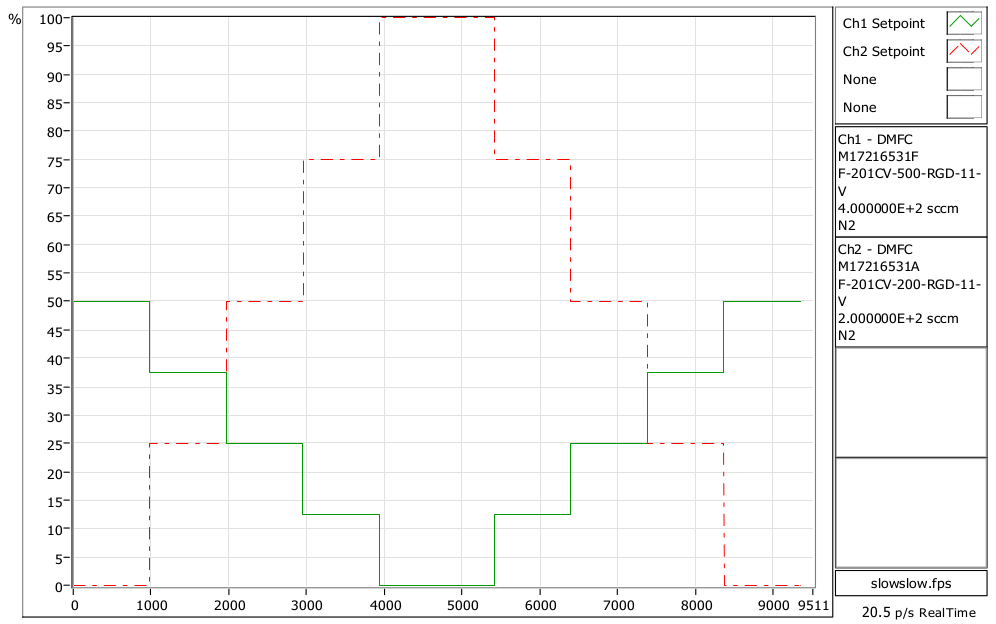
\includegraphics[width=\textwidth]{slowslowprotocol.png}
\caption{Slow swelling and slow deswelling protocol. Along the x-axis it shows the time in seconds, with the full SVA protocol taking $\SI{9500}{\second}$. Along the y-axis i show the precentage the mass flow meters are working at. The green plot belongs to the $400$SCCM Bronkhorst mass flow meter controlling the nitrogen gas and the red dashed plot belongs to the $200$SCCM Bronkhorst mass flow meter controlling the nitrogen flowing through the bubbler. The swelling is done by loading a swelling script called slowslow.fps and this script is show in appendix \ref{app:slowslow}.}
\label{fig:slowslow}
\end{figure}
   



\end{document}